\documentclass{standalone}
\usepackage{tikz}
\usetikzlibrary{patterns, positioning}


\begin{document}
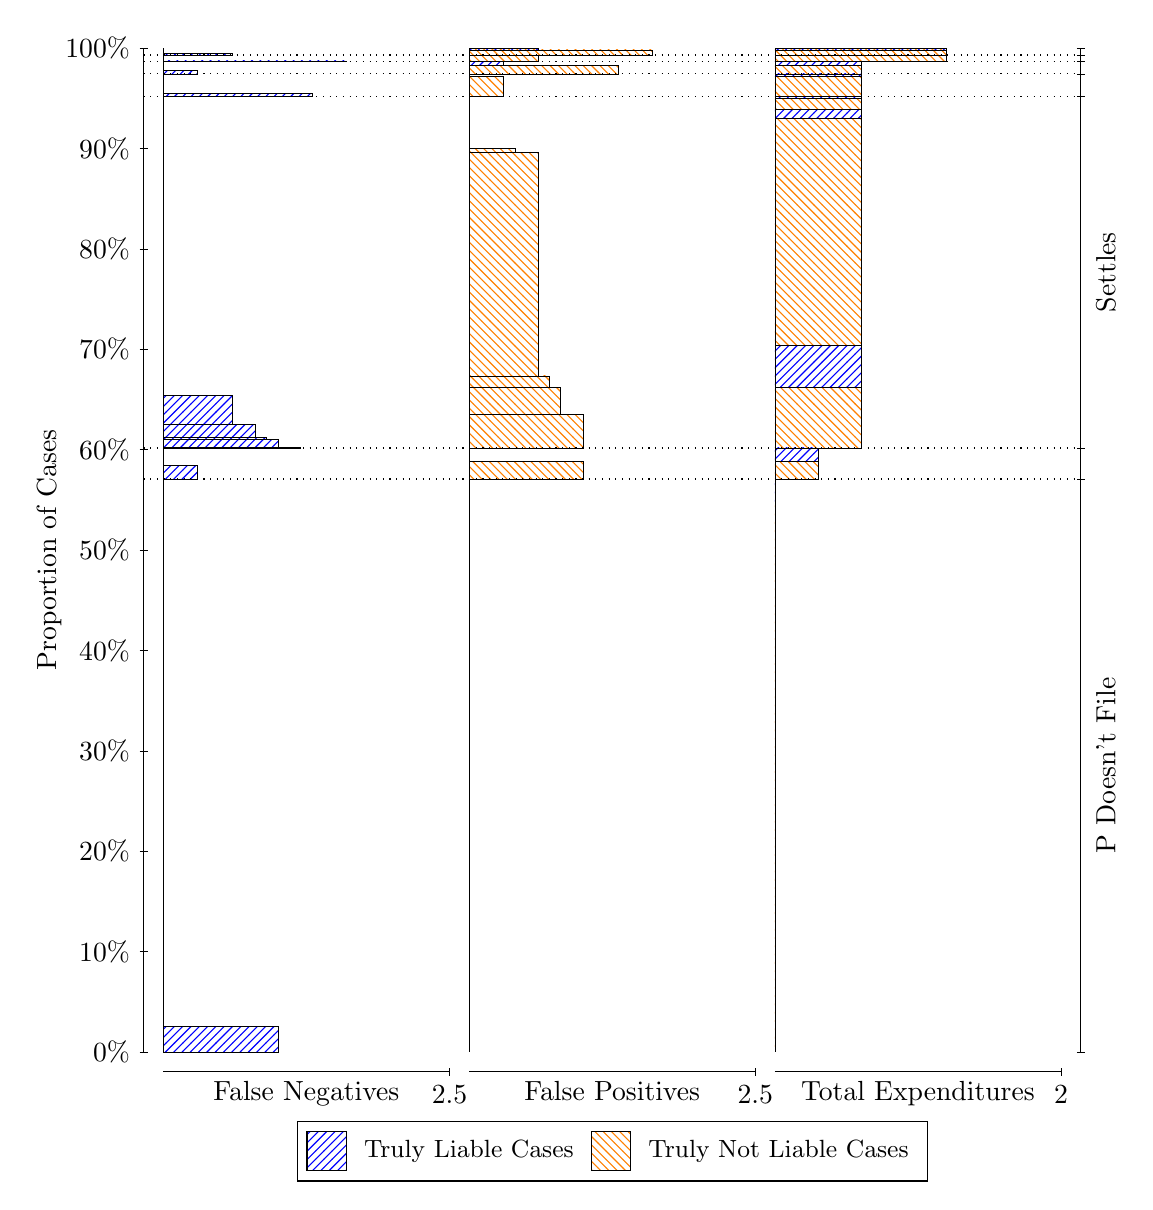
\begin{tikzpicture}
\draw[black, very thin] (1.5,1.75) -- (1.5,14.5);
\node[rotate=90, text=black, anchor=center] at (0.3, 8.125) {Proportion of Cases};
\draw[black, very thin] (1.45,1.75) -- (1.55,1.75);
\node[text=black, anchor=east] at (1.45, 1.75) {0\%};
\draw[black, very thin] (1.45,3.025) -- (1.55,3.025);
\node[text=black, anchor=east] at (1.45, 3.025) {10\%};
\draw[black, very thin] (1.45,4.3) -- (1.55,4.3);
\node[text=black, anchor=east] at (1.45, 4.3) {20\%};
\draw[black, very thin] (1.45,5.575) -- (1.55,5.575);
\node[text=black, anchor=east] at (1.45, 5.575) {30\%};
\draw[black, very thin] (1.45,6.85) -- (1.55,6.85);
\node[text=black, anchor=east] at (1.45, 6.85) {40\%};
\draw[black, very thin] (1.45,8.125) -- (1.55,8.125);
\node[text=black, anchor=east] at (1.45, 8.125) {50\%};
\draw[black, very thin] (1.45,9.4) -- (1.55,9.4);
\node[text=black, anchor=east] at (1.45, 9.4) {60\%};
\draw[black, very thin] (1.45,10.675) -- (1.55,10.675);
\node[text=black, anchor=east] at (1.45, 10.675) {70\%};
\draw[black, very thin] (1.45,11.95) -- (1.55,11.95);
\node[text=black, anchor=east] at (1.45, 11.95) {80\%};
\draw[black, very thin] (1.45,13.225) -- (1.55,13.225);
\node[text=black, anchor=east] at (1.45, 13.225) {90\%};
\draw[black, very thin] (1.45,14.5) -- (1.55,14.5);
\node[text=black, anchor=east] at (1.45, 14.5) {100\%};

\draw[black, very thin] (13.4,1.75) -- (13.4,14.5);
\draw[black, very thin] (13.35,1.75) -- (13.45,1.75);
\node[anchor=west] at (13.35, 1.75) {};
\draw[black, very thin] (13.35,9.0264) -- (13.45,9.0264);
\node[anchor=west] at (13.35, 9.0264) {};
\draw[black, very thin] (13.35,9.4205) -- (13.45,9.4205);
\node[anchor=west] at (13.35, 9.4205) {};
\draw[black, very thin] (13.35,13.887) -- (13.45,13.887);
\node[anchor=west] at (13.35, 13.887) {};
\draw[black, very thin] (13.35,14.172) -- (13.45,14.172);
\node[anchor=west] at (13.35, 14.172) {};
\draw[black, very thin] (13.35,14.329) -- (13.45,14.329);
\node[anchor=west] at (13.35, 14.329) {};
\draw[black, very thin] (13.35,14.411) -- (13.45,14.411);
\node[anchor=west] at (13.35, 14.411) {};
\draw[black, very thin] (13.35,14.5) -- (13.45,14.5);
\node[anchor=west] at (13.35, 14.5) {};

\draw[black, very thin, pattern color=blue, pattern=north east lines] (1.75,1.75) rectangle (3.2033,2.0767);
\draw[black, very thin, pattern color=orange, pattern=north west lines] (1.75,2.0767) rectangle (1.75,9.0264);
\draw[black, very thin, pattern color=blue, pattern=north east lines] (1.75,9.0264) rectangle (2.186,9.198);
\draw[black, very thin, pattern color=orange, pattern=north west lines] (1.75,9.198) rectangle (1.75,9.4205);
\draw[black, very thin, pattern color=blue, pattern=north east lines] (1.75,9.4205) rectangle (3.494,9.4261);
\draw[black, very thin, pattern color=blue, pattern=north east lines] (1.75,9.4261) rectangle (3.2033,9.5256);
\draw[black, very thin, pattern color=blue, pattern=north east lines] (1.75,9.5256) rectangle (3.058,9.5512);
\draw[black, very thin, pattern color=blue, pattern=north east lines] (1.75,9.5512) rectangle (2.9127,9.7178);
\draw[black, very thin, pattern color=blue, pattern=north east lines] (1.75,9.7178) rectangle (2.622,10.084);
\draw[black, very thin, pattern color=orange, pattern=north west lines] (1.75,10.084) rectangle (1.75,13.887);
\draw[black, very thin, pattern color=blue, pattern=north east lines] (1.75,13.887) rectangle (3.6393,13.92);
\draw[black, very thin, pattern color=orange, pattern=north west lines] (1.75,13.92) rectangle (1.75,14.172);
\draw[black, very thin, pattern color=blue, pattern=north east lines] (1.75,14.172) rectangle (2.186,14.22);
\draw[black, very thin, pattern color=orange, pattern=north west lines] (1.75,14.22) rectangle (1.75,14.329);
\draw[black, very thin, pattern color=blue, pattern=north east lines] (1.75,14.329) rectangle (4.0753,14.336);
\draw[black, very thin, pattern color=orange, pattern=north west lines] (1.75,14.336) rectangle (1.75,14.411);
\draw[black, very thin, pattern color=blue, pattern=north east lines] (1.75,14.411) rectangle (2.622,14.436);
\draw[black, very thin, pattern color=orange, pattern=north west lines] (1.75,14.436) rectangle (1.75,14.5);
\draw[black, very thin, pattern color=orange, pattern=north west lines] (5.6333,1.75) rectangle (5.6333,8.6997);
\draw[black, very thin, pattern color=blue, pattern=north east lines] (5.6333,8.6997) rectangle (5.6333,9.0264);
\draw[black, very thin, pattern color=orange, pattern=north west lines] (5.6333,9.0264) rectangle (7.0867,9.2489);
\draw[black, very thin, pattern color=blue, pattern=north east lines] (5.6333,9.2489) rectangle (5.6333,9.4205);
\draw[black, very thin, pattern color=orange, pattern=north west lines] (5.6333,9.4205) rectangle (7.0867,9.8446);
\draw[black, very thin, pattern color=orange, pattern=north west lines] (5.6333,9.8446) rectangle (6.796,10.193);
\draw[black, very thin, pattern color=orange, pattern=north west lines] (5.6333,10.193) rectangle (6.6507,10.337);
\draw[black, very thin, pattern color=orange, pattern=north west lines] (5.6333,10.337) rectangle (6.5053,13.174);
\draw[black, very thin, pattern color=orange, pattern=north west lines] (5.6333,13.174) rectangle (6.2147,13.223);
\draw[black, very thin, pattern color=blue, pattern=north east lines] (5.6333,13.223) rectangle (5.6333,13.887);
\draw[black, very thin, pattern color=orange, pattern=north west lines] (5.6333,13.887) rectangle (6.0693,14.139);
\draw[black, very thin, pattern color=blue, pattern=north east lines] (5.6333,14.139) rectangle (5.6333,14.172);
\draw[black, very thin, pattern color=orange, pattern=north west lines] (5.6333,14.172) rectangle (7.5227,14.281);
\draw[black, very thin, pattern color=blue, pattern=north east lines] (5.6333,14.281) rectangle (6.0693,14.329);
\draw[black, very thin, pattern color=orange, pattern=north west lines] (5.6333,14.329) rectangle (6.5053,14.404);
\draw[black, very thin, pattern color=blue, pattern=north east lines] (5.6333,14.404) rectangle (5.6333,14.411);
\draw[black, very thin, pattern color=orange, pattern=north west lines] (5.6333,14.411) rectangle (7.9587,14.475);
\draw[black, very thin, pattern color=blue, pattern=north east lines] (5.6333,14.475) rectangle (6.5053,14.5);
\draw[black, very thin, pattern color=orange, pattern=north west lines] (9.5167,1.75) rectangle (9.5167,8.6997);
\draw[black, very thin, pattern color=blue, pattern=north east lines] (9.5167,8.6997) rectangle (9.5167,9.0264);
\draw[black, very thin, pattern color=orange, pattern=north west lines] (9.5167,9.0264) rectangle (10.062,9.2489);
\draw[black, very thin, pattern color=blue, pattern=north east lines] (9.5167,9.2489) rectangle (10.062,9.4205);
\draw[black, very thin, pattern color=orange, pattern=north west lines] (9.5167,9.4205) rectangle (10.607,10.193);
\draw[black, very thin, pattern color=blue, pattern=north east lines] (9.5167,10.193) rectangle (10.607,10.725);
\draw[black, very thin, pattern color=orange, pattern=north west lines] (9.5167,10.725) rectangle (10.607,13.612);
\draw[black, very thin, pattern color=blue, pattern=north east lines] (9.5167,13.612) rectangle (10.607,13.717);
\draw[black, very thin, pattern color=orange, pattern=north west lines] (9.5167,13.717) rectangle (10.607,13.861);
\draw[black, very thin, pattern color=blue, pattern=north east lines] (9.5167,13.861) rectangle (10.607,13.887);
\draw[black, very thin, pattern color=orange, pattern=north west lines] (9.5167,13.887) rectangle (10.607,14.139);
\draw[black, very thin, pattern color=blue, pattern=north east lines] (9.5167,14.139) rectangle (10.607,14.172);
\draw[black, very thin, pattern color=orange, pattern=north west lines] (9.5167,14.172) rectangle (10.607,14.281);
\draw[black, very thin, pattern color=blue, pattern=north east lines] (9.5167,14.281) rectangle (10.607,14.329);
\draw[black, very thin, pattern color=orange, pattern=north west lines] (9.5167,14.329) rectangle (11.697,14.404);
\draw[black, very thin, pattern color=blue, pattern=north east lines] (9.5167,14.404) rectangle (11.697,14.411);
\draw[black, very thin, pattern color=orange, pattern=north west lines] (9.5167,14.411) rectangle (11.697,14.475);
\draw[black, very thin, pattern color=blue, pattern=north east lines] (9.5167,14.475) rectangle (11.697,14.5);
\draw[black, dotted] (1.5,9.0264) -- (13.4,9.0264);
\draw[black, dotted] (1.5,9.4205) -- (13.4,9.4205);
\draw[black, dotted] (1.5,13.887) -- (13.4,13.887);
\draw[black, dotted] (1.5,14.172) -- (13.4,14.172);
\draw[black, dotted] (1.5,14.329) -- (13.4,14.329);
\draw[black, dotted] (1.5,14.411) -- (13.4,14.411);
\draw[black, very thin] (1.75,1.5) -- (5.3833,1.5);
\node[text=black, anchor=north] at (3.5667, 1.5) {False Negatives};
\draw[black, very thin] (5.3833,1.45) -- (5.3833,1.55);
\node[text=black, anchor=north] at (5.3833, 1.45) {2.5};

\draw[black, very thin] (5.6333,1.5) -- (9.2667,1.5);
\node[text=black, anchor=north] at (7.45, 1.5) {False Positives};
\draw[black, very thin] (9.2667,1.45) -- (9.2667,1.55);
\node[text=black, anchor=north] at (9.2667, 1.45) {2.5};

\draw[black, very thin] (9.5167,1.5) -- (13.15,1.5);
\node[text=black, anchor=north] at (11.333, 1.5) {Total Expenditures};
\draw[black, very thin] (13.15,1.45) -- (13.15,1.55);
\node[text=black, anchor=north] at (13.15, 1.45) {2};

\node[text=black, centered, rotate=90] at (13.72, 5.3882) {P Doesn't File};

\node[text=black, centered, rotate=90] at (13.72, 11.654) {Settles};





\draw (7.449999999999999,1.5) node[draw=none] (baseCoordinate) {};
\begin{scope}[align=center]
        \matrix[scale=0.5, draw=black, below=0.5cm of baseCoordinate, nodes={draw}, column sep=0.1cm]{
            \node[rectangle, draw, minimum width=0.5cm, minimum height=0.5cm, pattern color=blue, pattern=north east lines] {}; &
            \node[draw=none, font=\small, text=black] (B) {Truly Liable Cases}; &
            \node[rectangle, draw, minimum width=0.5cm, minimum height=0.5cm, pattern color=orange, pattern=north west lines] {}; &
            \node[draw=none, font=\small, text=black] (B) {Truly Not Liable Cases}; \\
            };
\end{scope}

\end{tikzpicture}
\end{document}